\subsection{Spatial Pooler}


\begin{frame}[c]{Spatial Pooler - Introduction}
    \pause
                                     % trim = left bottom right top
    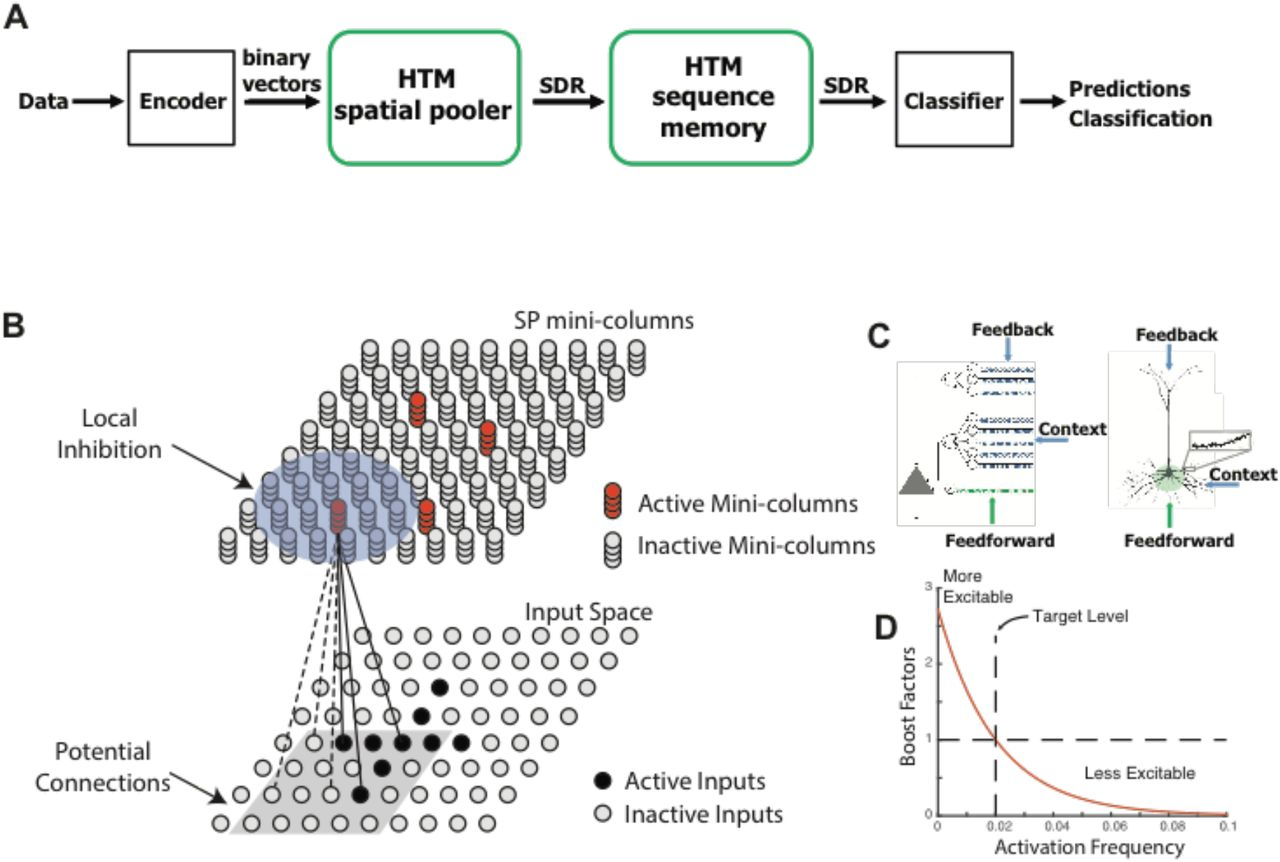
\includegraphics[width=\textwidth, trim= 0 0 97 70, clip]{spatial_pooler} \\
    \normalsize
    Image adapted from \cite{cui2017htm}.
\end{frame}


\begin{frame}[c,fragile]{Spatial Pooler - Connection details}
    \Large
    Show \verb!Ep8/Learning Rules!!
    \newline
    \begin{itemize}[<+(1)->]
        \item Many Connections
        \item Only Columns with highest overlap scores continue
        \item Everyone else gets inhibited
        \item Next: Updating Permanence Values
    \end{itemize}
\end{frame}


\begin{frame}[c,allowframebreaks]{Spatial Pooler - Learning Details}
    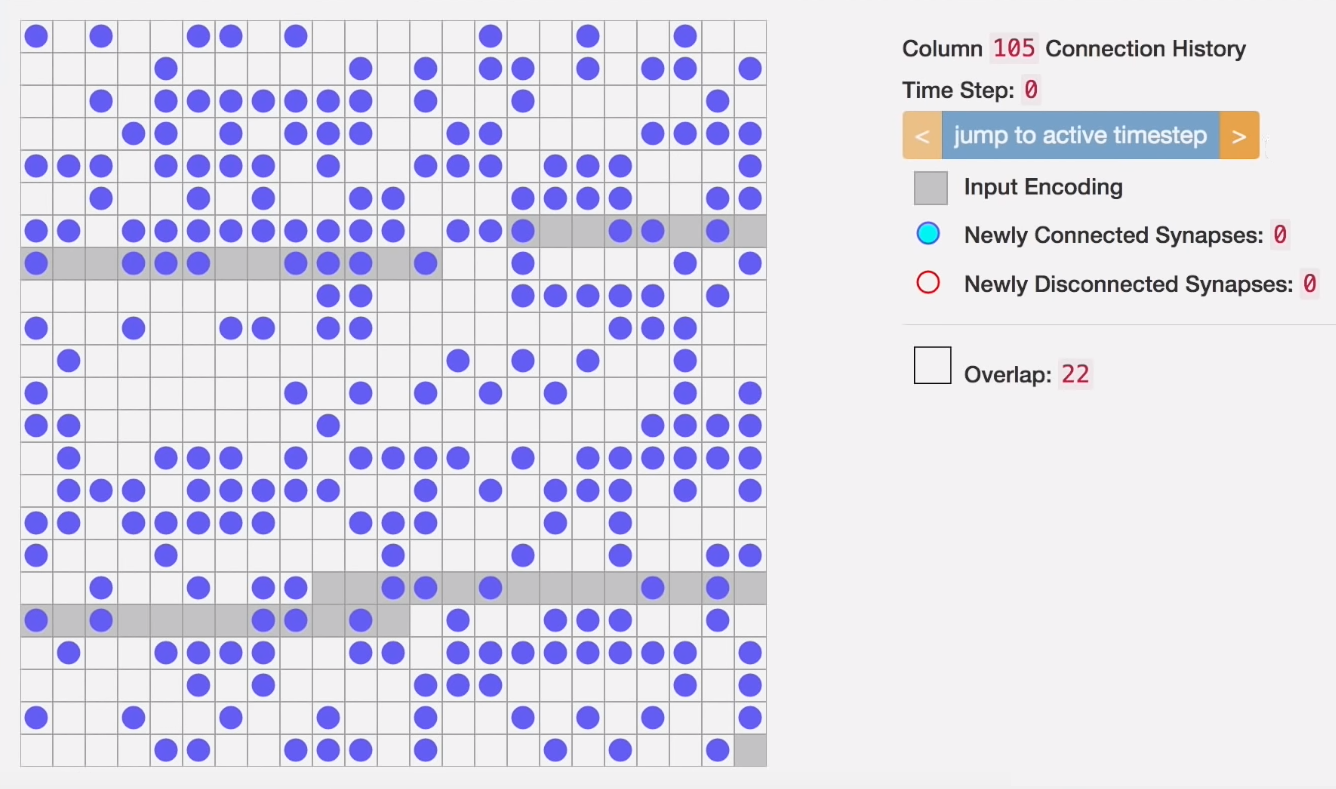
\includegraphics[width=\textwidth]{learn_ex5}
    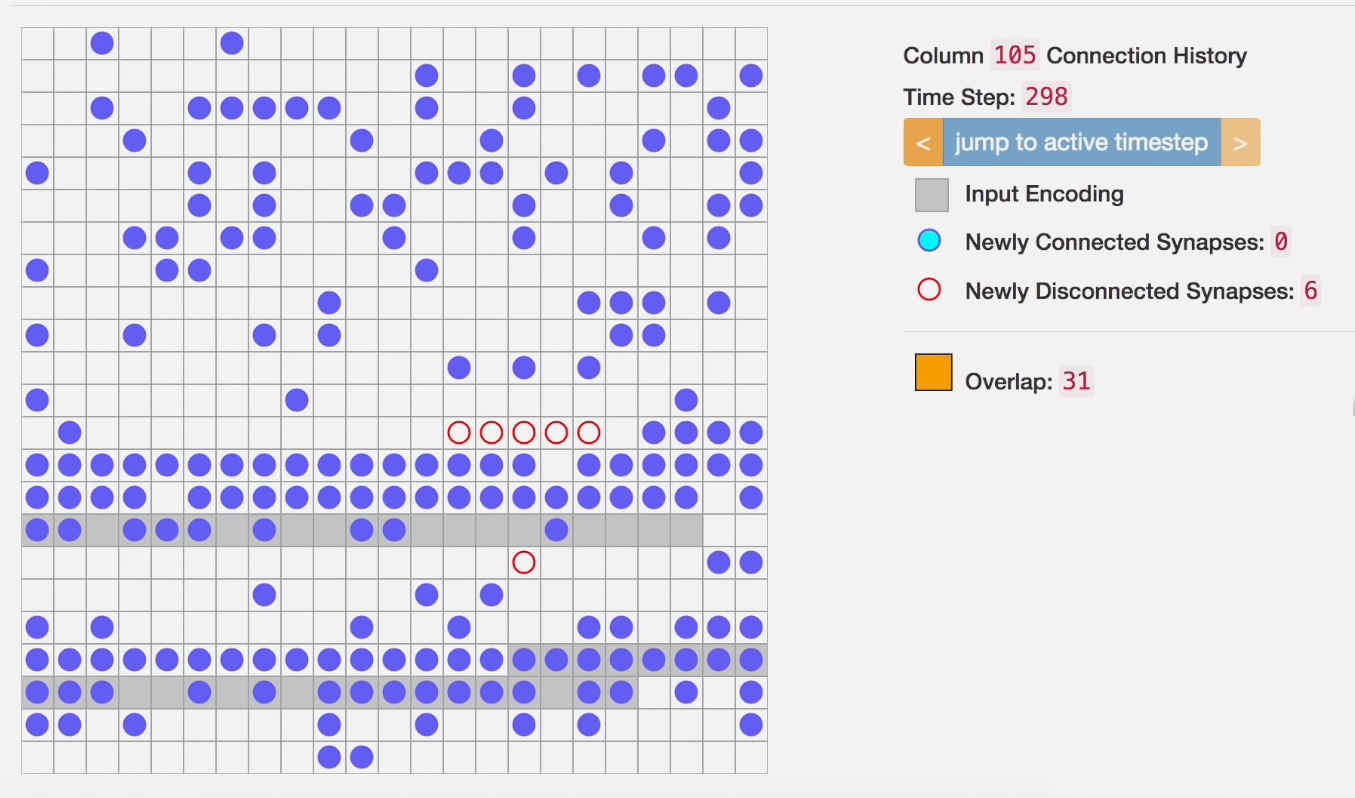
\includegraphics[width=\textwidth]{learn_ex3}
    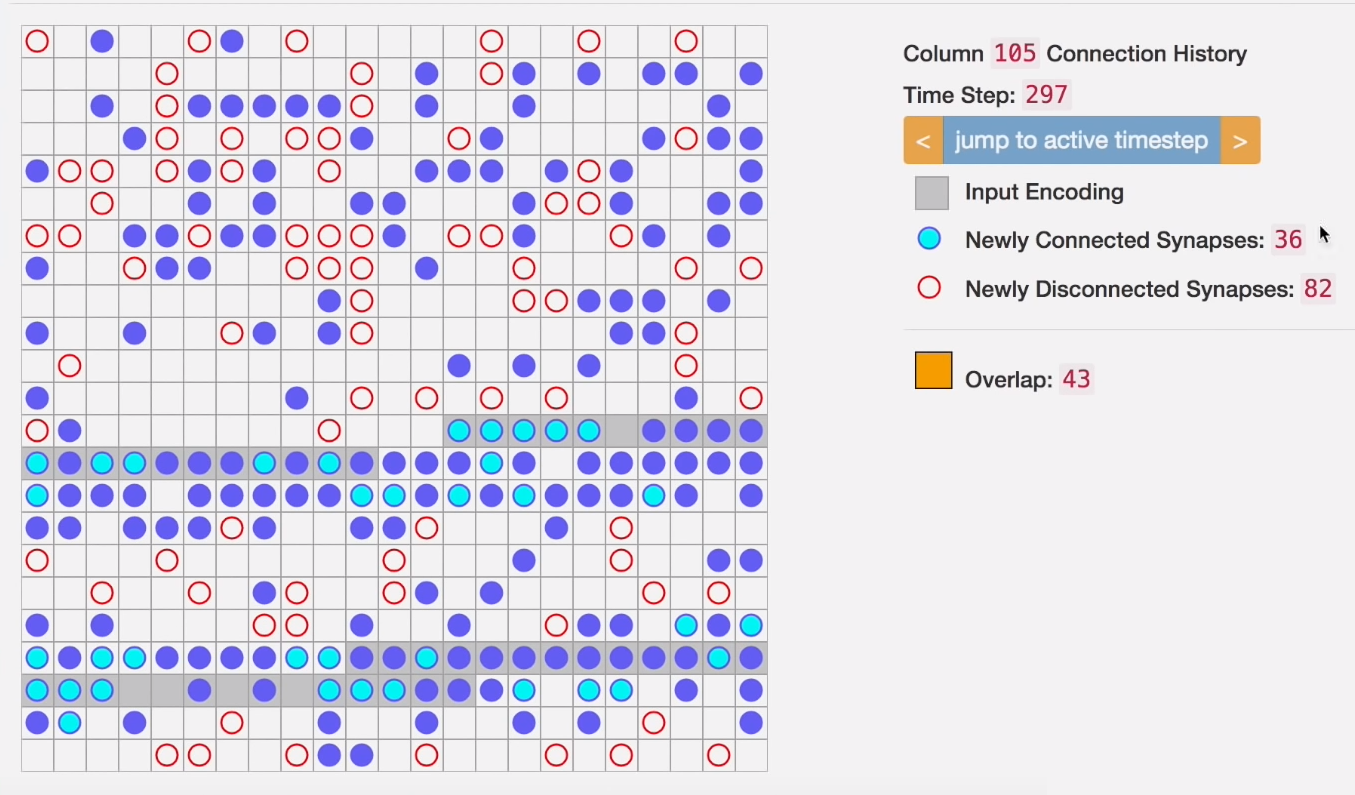
\includegraphics[width=\textwidth]{learn_ex2}
    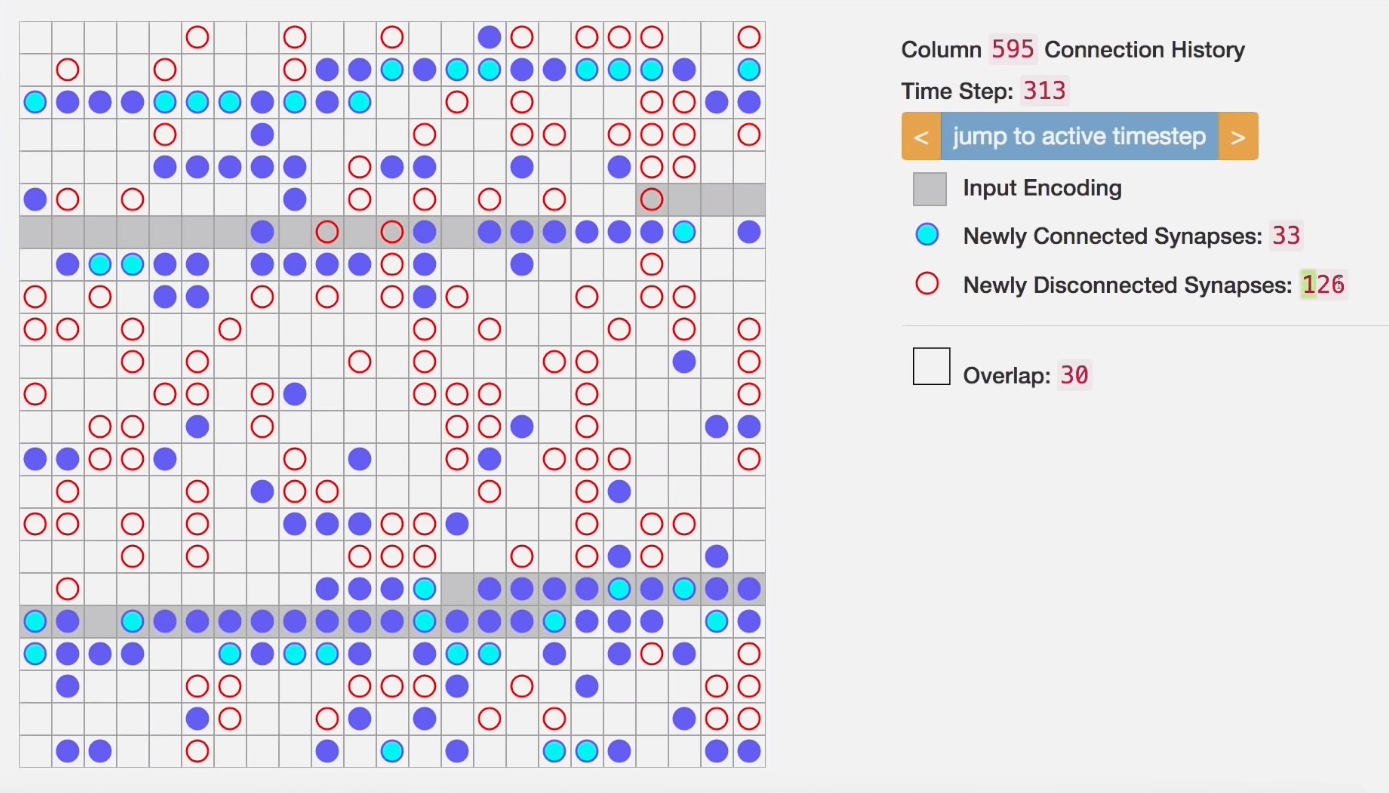
\includegraphics[width=\textwidth]{learn_ex1}
\end{frame}



% Show Pictures about granularity with vs without boosting, explain that with boosting more cells start to represent slightly different concepts


\begin{frame}[c,allowframebreaks]{Spatial Pooler - Boosting}
    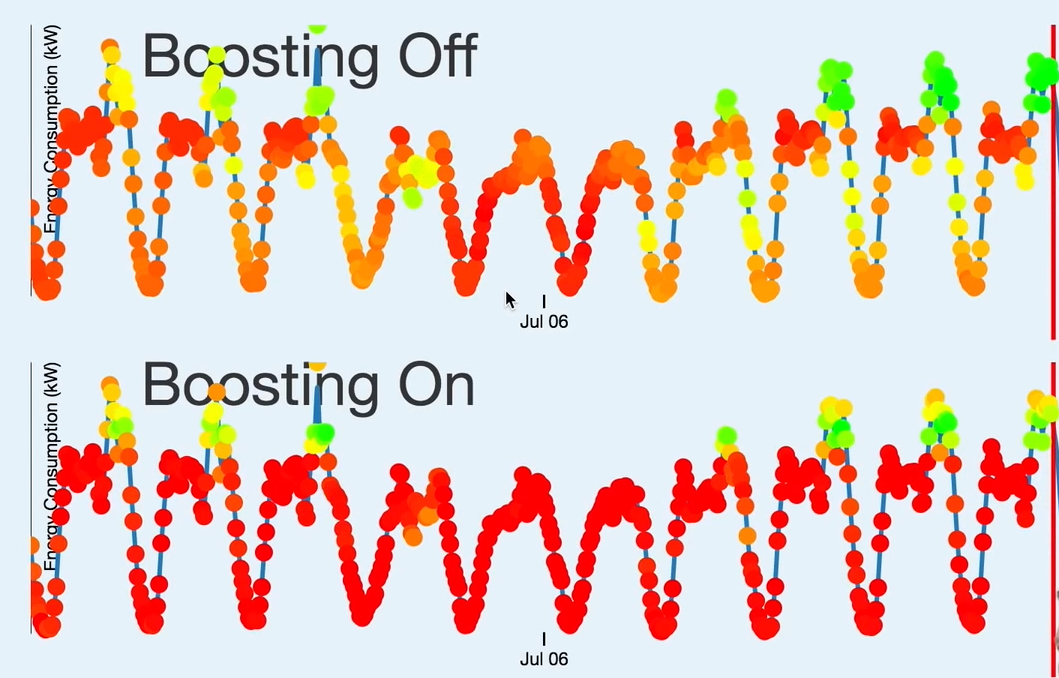
\includegraphics[width=\textwidth]{boost_ex1}
    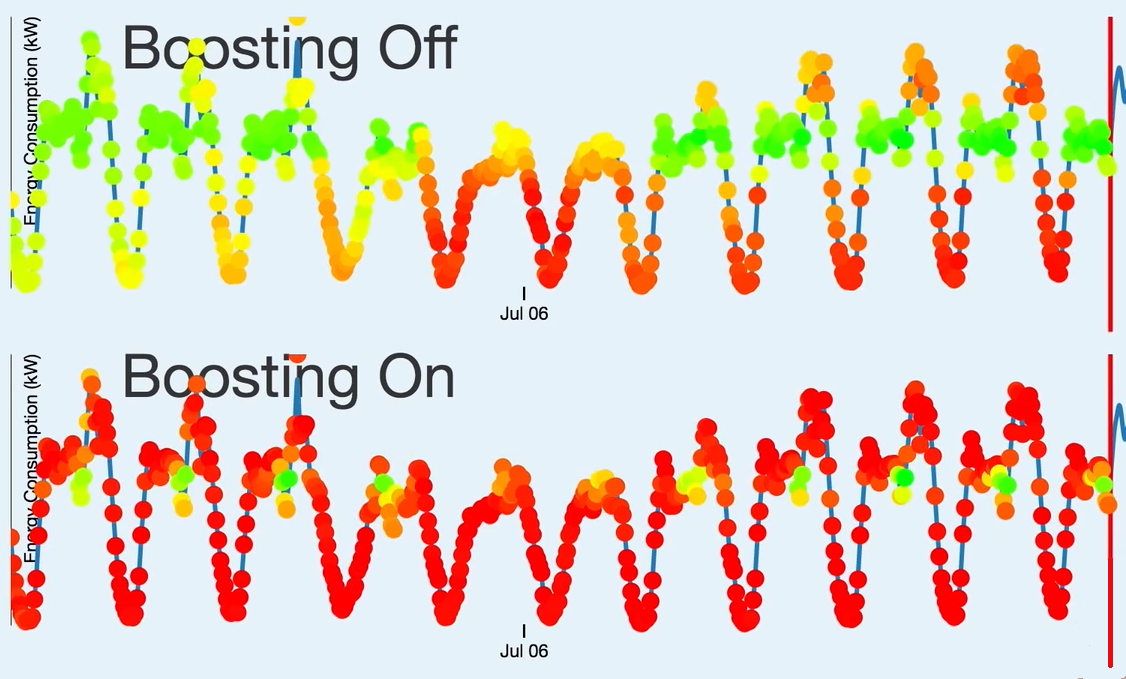
\includegraphics[width=\textwidth]{boost_ex2}
    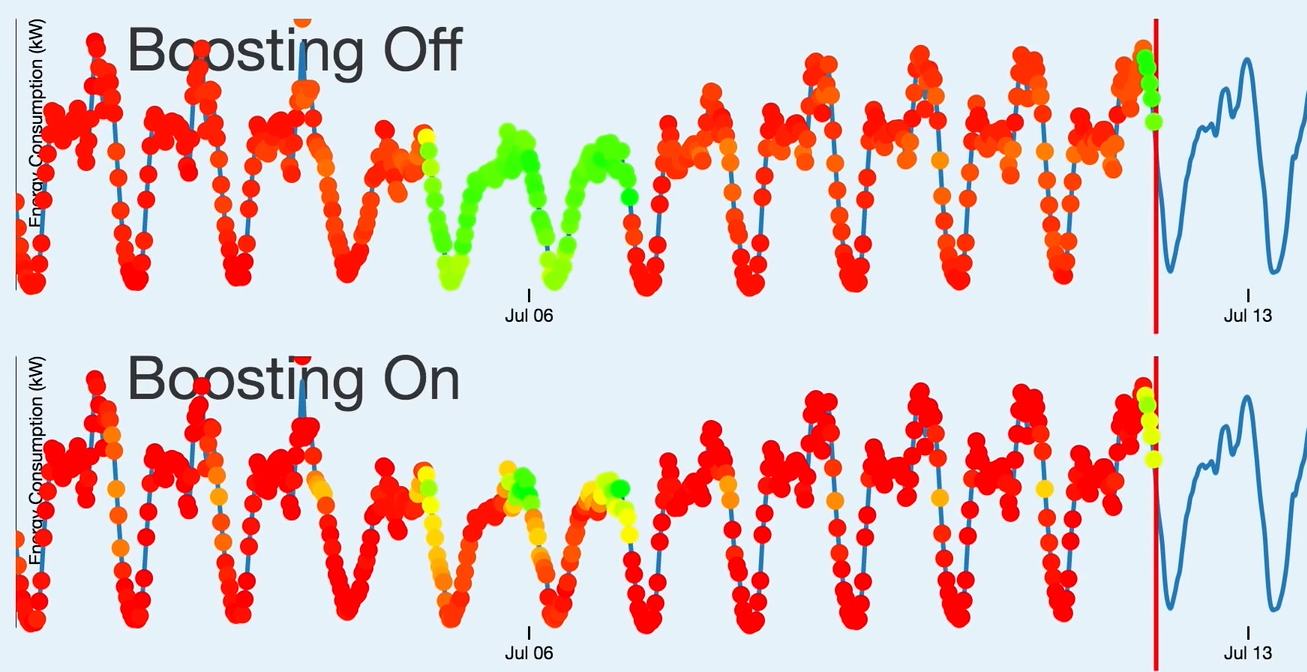
\includegraphics[width=\textwidth]{boost_ex3}
\end{frame}


\begin{frame}[c]{Spatial Pooler - Parameters}
    \Large
    \begin{itemize}[<+(1)->]
        \item Algorithm Structure (receptive field)
        \item Inhibition
        \item Learning rates
        \item Column Activity
    \end{itemize}
\end{frame}


\begin{frame}[c]{Spatial Pooler - Phases}
    \Large
    \begin{enumerate}[<+(1)->]
        \item Initializing with random variables
        \item Compute overlap scores (+Boost)
        \item Inhibition
        \item Updating Permanence values
        \item Repeat from step 2 with new input
    \end{enumerate}
\end{frame}






% SPATIAL POOLER STEPS
% 
% 1. Start with an input consisting of a fixed number of bits. These bits might
% represent sensory data or they might come from another region elsewhere in the
% HTM system.
% 
% 2. Initialize the HTM region by assigning a fixed number of columns to the
% region receiving this input. Each column has an associated dendritic segment,
% serving as the connection to the input space. Each dendrite segment has a set
% of potential synapses representing a (random) subset of the input bits. Each
% potential synapse has a permanence value. These values are randomly initialized
% around the permanence threshold. Based on their permanence values, some of the
% potential synapses will already be connected; the permanences are greater than
% than the threshold value.
% 
% 3. For any given input, determine how many connected synapses on each column
% are connected to active (ON) input bits. These are active synapses.
% 
% 4. The number of active synapses is multiplied by a “boosting” factor, which is
% dynamically determined by how often a column is active relative to its
% neighbors.
% 
% 5. A small percentage of columns within the inhibition radius with the highest
% activations (after boosting) become active, and disable the other columns
% within the radius. The inhibition radius is itself dynamically determined by
% the spread of input bits. There is now a sparse set of active columns.
% 
% 6. The region now follows the Spatial Pooling (Hebbian-style) learning rule:
% For each of the active columns, we adjust the permanence values of all the
% potential synapses. The permanence values of synapses aligned with active input
% bits are increased. The permanence values of synapses aligned with inactive
% input bits are decreased. The changes made to permanence values may change some
% synapses from being connected to unconnected, and vice-versa.
% 
% 7. For subsequent inputs, we repeat from step 3.


% \cite{cui2017htm} % <- spatial pooler



